\documentclass[11pt]{article}
\usepackage[a4paper,margin=2.6cm]{geometry}
\usepackage[T1]{fontenc}
\usepackage{lmodern}
\usepackage{amsmath,amssymb,amsthm,mathtools}
\usepackage{booktabs}
\usepackage{graphicx}
\usepackage[round]{natbib}
\usepackage{enumitem}
\usepackage[hidelinks]{hyperref}
\usepackage{xcolor}

\newtheorem{theorem}{Theorem}
\newtheorem{proposition}{Proposition}
\newtheorem{lemma}{Lemma}
\newtheorem{corollary}{Corollary}
\theoremstyle{definition}
\newtheorem{definition}{Definition}
\newtheorem{remark}{Remark}
\newtheorem{example}{Example}

\newcommand{\E}{\mathbb{E}}
\renewcommand{\P}{\mathbb{P}}
\newcommand{\ind}{\mathbf{1}}
\newcommand{\Y}{\mathcal{Y}}
\newcommand{\X}{\mathcal{X}}

\title{Confidently Wrong: Limits of Sampling-Based Confidence\\for Abstaining LLM Agents}
\author{Le Nam Khanh\\[2pt]
\small Department of Data Science and Artificial Intelligence\\
\small The Hong Kong Polytechnic University}
\date{Technical note, November 2026}

\begin{document}
\maketitle

\begin{abstract}
Agents built on large language models are increasingly asked to abstain, or to state a
confidence, when they might be wrong. The cheapest confidence signals are computed from repeated
runs: majority agreement (self-consistency), semantic entropy, and their relatives. We study the
whole class of such \emph{label-invariant} scores, those that depend only on which runs agree with
which. We show that, given the agent's output distribution on a task, these scores carry no
information about whether its preferred answer is correct. As a consequence, tasks on which the
agent is deterministic form a blind spot: if a share $\pi_D$ of tasks are deterministic and a
fraction $\rho$ of those are answered wrongly, every abstention policy that trusts unanimity at
least as much as anything else has selective risk at least $\pi_D\rho$, at every coverage and for
every number of runs. No calibration procedure, however much labelled data it uses, can then
certify a risk level below $\pi_D\rho$: a valid procedure abstains on everything. In a binary model
we give the risk--coverage curve in closed form and show that, as the number of runs grows,
agreement reveals \emph{how strongly} the agent prefers an answer but never \emph{whether} it is the
right one. Breaking the floor needs a second source of evidence whose errors are less correlated
with the agent's than its correct answers are. Finally, the same quantity that drives the floor,
the intra-task correlation of errors, inflates the variance of agent evaluations by the design
effect $1+(k-1)\,\mathrm{ICC}$. All closed forms are checked by simulation in the accompanying code.
\end{abstract}

\section{Introduction}

A data-analysis agent asked whether a regression coefficient is significant, or a question
answering system asked for a fact, should sometimes decline, or answer with an honest
confidence. Because language models are stochastic, a natural confidence signal is obtained by
running the model $k$ times and measuring how much the runs agree: majority voting, or
self-consistency \citep{wang2023selfconsistency}, semantic entropy over clusters of equivalent
answers \citep{kuhn2023semantic,farquhar2024detecting}, and consistency checks between samples
\citep{manakul2023selfcheckgpt}. Calibration frameworks then turn such a score into an abstention
rule with a finite-sample guarantee on the error rate among answered questions
\citep{angelopoulos2021ltt,angelopoulos2024crc,yadkori2024conformal}.

A failure mode of these signals is widely reported: a model can give the same wrong answer on
every run, so that agreement is maximal precisely where the answer is wrong
\citep{phillips2026entropy,hamidieh2026complementing,ding2026agree,kossen2024probes}. This note
makes that observation precise and quantitative, and works out what it implies for abstention,
for certification and for evaluation.

\paragraph{Contributions.}
\begin{enumerate}[leftmargin=*,itemsep=2pt]
\item \textbf{Profile sufficiency} (Lemma~\ref{lem:profile}). For any score that depends only on
which runs agree, the joint law of the score and of the correctness of the majority answer
depends on the task only through the sorted output probabilities and the rank of the correct
answer among them; the score is independent of that rank.
\item \textbf{The deterministic blind spot} (Theorem~\ref{thm:floor}). Three lower bounds on the
selective risk of label-invariant abstention policies, in terms of the mass $\pi_D$ of
deterministic tasks and the share $\rho$ of them that are wrong. Corollaries: certification below
$\pi_D\rho$ is impossible, the certifiable coverages form a window that may be empty, and a
calibrated label-invariant confidence must report $1-\rho$ on every deterministic task.
\item \textbf{Binary model} (Proposition~\ref{prop:binary}). Closed-form risk--coverage curves
and their limit as $k\to\infty$: agreement estimates $|2A-1|$, where $A$ is the per-run accuracy,
while correctness is $\operatorname{sign}(2A-1)$.
\item \textbf{Breaking the floor} (Proposition~\ref{prop:second}). A second source helps if and
only if it agrees with the agent's wrong answers less often than with its right ones.
\item \textbf{Certification and evaluation} (Propositions~\ref{prop:ltt} and \ref{prop:eval}).
A fixed-sequence binomial test that is valid and, by Theorem~\ref{thm:floor}, abstains on
everything when it must; a sample-size rule; and the design effect of evaluating agents with
several runs per task, governed by the same intra-task correlation.
\end{enumerate}
The results are elementary; their purpose is to state exactly which guarantees sampling-based
confidence can and cannot deliver, so that abstention and evaluation can be designed around them.

\section{Setting}\label{sec:setting}

Tasks $X\sim P$ take values in $\X$; task $x$ has a correct answer $y^\star(x)$ in a countable
answer space $\Y$ (for free-form answers, $\Y$ can be a set of semantic equivalence classes). A run
of the agent on $x$ returns $Y\sim Q_x$, and runs are independent given the task. With $k$ runs
$Y_{1:k}$ the agent reports the plurality answer $M$, breaking ties uniformly at random, and we
write $C=\ind\{M=y^\star(X)\}$ for its correctness.

A \emph{score} is $S=g(Y_{1:k})$ for a measurable $g$. A \emph{policy} $\varphi$ answers with
probability $\varphi(S)\in[0,1]$, using randomness independent of everything else. Its coverage and
selective risk are
\[
c(\varphi)=\E\,\varphi(S),\qquad
R(\varphi)=\frac{\E\,[\varphi(S)(1-C)]}{c(\varphi)}.
\]

\begin{definition}[label invariance]
A score $g$ is \emph{label-invariant} if $g(\sigma\circ y_{1:k})=g(y_{1:k})$ for every bijection
$\sigma$ of $\Y$ and $g(y_{\tau(1)},\dots,y_{\tau(k)})=g(y_{1:k})$ for every permutation $\tau$ of
$\{1,\dots,k\}$. Equivalently, $g$ depends on $y_{1:k}$ only through the multiset of the sizes of
its blocks of equal answers.
\end{definition}

Majority agreement $\max_y \#\{t:y_t=y\}/k$, the number of distinct answers, the empirical
entropy of the answer frequencies, semantic entropy over equivalence classes, and the rate of
pairwise agreement between runs are all label-invariant. Verbalised confidence, token
probabilities, verifier or judge scores, probes of hidden states, and anything computed from a
second model are not.

\paragraph{Profiles.} Order the atoms of $Q_x$ by decreasing mass,
$a_1(x)\ge a_2(x)\ge\dots$, breaking ties by a fixed order on $\Y$, and let $\nu_x(r)$ be the answer
of rank $r$. The \emph{profile} of $x$ is $\Pi(x)=(a_1(x),a_2(x),\dots)$ and $J(x)$ is the rank of the
correct answer ($J(x)=\infty$ if $Q_x(y^\star(x))=0$). A task is \emph{deterministic} if $a_1(x)=1$; let
\[
D=\{x:a_1(x)=1\},\quad \pi_D=\P(X\in D),\quad \rho=\P(C=0\mid X\in D)=\P(J(X)\neq 1\mid X\in D).
\]
$\rho$ is the share of deterministic tasks whose only answer is wrong: the agent's
\emph{systematic} errors. Let $u$ be the block structure in which all $k$ runs agree and
$\P(U)=\E\sum_r a_r(X)^k$ the probability of unanimity.

\section{Profile sufficiency}

\begin{lemma}[profile sufficiency]\label{lem:profile}
Let $g$ be label-invariant and let $R_M$ be the rank of the plurality answer. Conditional on
$X=x$, the law of $(S,R_M)$ depends on $x$ only through $\Pi(x)$. Hence $(S,R_M)$ is independent of
$X$ given $\Pi(X)$, in particular of $J(X)$, and $C=\ind\{R_M=J(X)\}$.
\end{lemma}

\begin{proof}
Fix $x$ and let $R_t=\nu_x^{-1}(Y_t)$ be the rank of run $t$'s answer. The $R_t$ are independent with
$\P(R_t=r)=a_r(x)$. Since $\nu_x$ is injective, $Y_t=Y_s$ if and only if $R_t=R_s$, so $Y_{1:k}$ and
$R_{1:k}$ have the same block structure and $S=h(R_{1:k})$ for the function $h$ through which $g$
factors. Ties in the plurality correspond one to one, so the plurality of $Y_{1:k}$ is
$\nu_x$ of the plurality of $R_{1:k}$ under the same uniform tie-break. Thus $(S,R_M)$ is a fixed
function of $R_{1:k}$ and independent tie-breaking randomness, and $R_{1:k}$ is i.i.d.\ from
$\Pi(x)$. Finally $M=y^\star(x)$ if and only if $\nu_x(R_M)=\nu_x(J(x))$.
\end{proof}

The lemma says that a label-invariant score sees the \emph{shape} of the agent's output
distribution and nothing else. Whether the agent's favourite answer is right is the rank $J$,
which the shape does not determine.

\section{The deterministic blind spot}

\begin{theorem}\label{thm:floor}
Let $g$ be label-invariant with value $s_u$ on unanimous runs, assume $\pi_D>0$, and let
$\varphi$ be a policy with coverage $c>0$.
\begin{enumerate}[label=(\alph*),itemsep=2pt]
\item For every policy, $R(\varphi)\ \ge\ \rho\,\dfrac{(c-(1-\pi_D))_+}{c}$.
\item If $\varphi(s_u)\ge\varphi(s)$ for all $s$ (unanimity is answered at least as readily as
anything else), then $R(\varphi)\ge\pi_D\,\rho$.
\item If $g(y)<s_u$ whenever $y$ is not unanimous and $\varphi$ is a threshold policy on $g$
(answer if $S>\lambda$, with probability $\gamma$ if $S=\lambda$), then
\[
R(\varphi)\ \ge\ \frac{\pi_D\,\rho}{\max\{c,\ \P(U)\}}.
\]
\end{enumerate}
The bounds hold for every $k$ and do not depend on how $\varphi$ was chosen.
\end{theorem}

\begin{proof}
On $D$ every run returns the same answer, so $S=s_u$ and the task is answered with probability
$\varphi(s_u)$, independently of $C$. Hence the answered mass from $D$ is $\varphi(s_u)\pi_D$ and the
wrong answered mass from $D$ is $\varphi(s_u)\pi_D\rho$, so
\begin{equation}\label{eq:basic}
R(\varphi)\ \ge\ \frac{\varphi(s_u)\,\pi_D\,\rho}{c}.
\end{equation}
(a) Tasks outside $D$ contribute at most $1-\pi_D$ to the coverage, so
$\varphi(s_u)\pi_D\ge c-(1-\pi_D)$. (b) $c=\E\,\varphi(S)\le\sup_s\varphi(s)=\varphi(s_u)$.
(c) If $c\le\P(U)$, only unanimous runs can be answered and $\varphi(s_u)=c/\P(U)$; if $c>\P(U)$,
some non-unanimous runs are answered, so $\lambda<s_u$ and $\varphi(s_u)=1$. Substitute into
\eqref{eq:basic}.
\end{proof}

Bound (a) applies to any policy, including perverse ones that distrust unanimity; it says that
covering more than the non-deterministic tasks forces deterministic errors into the answered set.
Bound (b) covers every policy built on the usual reading of agreement. Bound (c) is attained at
the unanimity threshold as $k\to\infty$: since $\P(U)\downarrow\pi_D$ (each non-degenerate
profile has $\sum_r a_r^k\to 0$), the unanimous answers of a large-$k$ agent are wrong at rate
$\rho$ whatever the rest of the population looks like.

\begin{remark}[near-deterministic tasks]
The same argument applies to $D_\epsilon=\{x:a_1(x)\ge 1-\epsilon\}$ with
$\rho_\epsilon=\P(J\neq 1\mid X\in D_\epsilon)$. On such a task with a wrong favourite answer,
all runs agree on that answer with probability at least $(1-\epsilon)^k$, so (b) becomes
$R(\varphi)\ge(1-\epsilon)^k\,\P(X\in D_\epsilon)\,\rho_\epsilon$.
\end{remark}

\begin{corollary}[certification]\label{cor:cert}
Fix a target $\alpha\in(0,1)$.
\begin{enumerate}[label=(\roman*),itemsep=2pt]
\item If $\pi_D\rho>\alpha$, no policy satisfying the condition of Theorem~\ref{thm:floor}(b) has
selective risk at most $\alpha$ at any positive coverage. A procedure that returns such a policy
with $\P(R\le\alpha)\ge 1-\delta$ must abstain on everything with probability at least $1-\delta$.
\item For threshold policies as in Theorem~\ref{thm:floor}(c) with $\pi_D\rho/\alpha>\P(U)$, risk
at most $\alpha$ requires $c\ge\pi_D\rho/\alpha$. Any policy also needs $c\le(1-\mu)/(1-\alpha)$,
where $\mu=1-\E C$ is the risk of answering everything, because abstaining removes at most
$1-c$ of the error mass \citep[the same bound appears in][]{kotte2026crc}. The certifiable coverages
therefore lie in
\[
\Big[\tfrac{\pi_D\rho}{\alpha},\ \tfrac{1-\mu}{1-\alpha}\Big],
\]
which is empty when $\pi_D\rho\,(1-\alpha)>\alpha\,(1-\mu)$.
\end{enumerate}
\end{corollary}

\begin{proof}
(i) is immediate from Theorem~\ref{thm:floor}(b): every candidate violates the target, so a
valid procedure may return one only with probability at most $\delta$. (ii) The lower end follows
from Theorem~\ref{thm:floor}(c). For the upper end, the error mass among answered tasks is at least
$\mu-(1-c)$, so $R\ge(\mu-1+c)/c$, which is at most $\alpha$ only if $c\le(1-\mu)/(1-\alpha)$.
\end{proof}

\begin{corollary}[honest confidence]\label{cor:conf}
Let $f$ map the score to a stated confidence in $[0,1]$. On $D$ the stated confidence is the
constant $f(s_u)$, so
\[
\E\big[(f(S)-C)^2\,\big|\,X\in D\big]=(1-\rho)(1-f(s_u))^2+\rho f(s_u)^2\ \ge\ \rho(1-\rho),
\]
with equality only if $f(s_u)=1-\rho$. If $f$ is calibrated, $f(s_u)=\P(C=1\mid U)$, which tends to
$1-\rho$ as $k\to\infty$.
\end{corollary}

An agent that reports confidence from its own agreement can therefore be calibrated, but it must
say the same number on every task it answers deterministically, and that number is $1-\rho$,
however unanimous the runs. The Brier score on deterministic tasks cannot fall below
$\rho(1-\rho)$: the resolution that would separate right from wrong deterministic answers is
simply not in the signal.

\section{A binary model}\label{sec:binary}

Many agent decisions are binary: significant or not, buy or sell, safe or unsafe. Let task $x$ have
two possible answers and let $A(x)=Q_x(y^\star(x))$ be the per-run accuracy. With $k$ odd, let
$N\sim\mathrm{Bin}(k,A)$ be the number of correct runs and $V=\max(N,k-N)$ the votes for the majority.
Every label-invariant score is a function of $V$, so every label-invariant policy is a function
$\varphi(V)$, and deterministic tasks are those with $A\in\{0,1\}$, with
$\rho=\P(A=0)/\P(A\in\{0,1\})$.

\begin{proposition}\label{prop:binary}
Answering when $V\ge m$, for $(k+1)/2\le m\le k$,
\[
c_k(m)=\E\big[\P(N\ge m\mid A)+\P(N\le k-m\mid A)\big],\qquad
R_k(m)=\frac{\E\,\P(N\le k-m\mid A)}{c_k(m)}.
\]
Let $k\to\infty$ with $m_k/k\to\lambda\in(\tfrac12,1)$ and $\P(|2A-1|=2\lambda-1)=0$. Then
\[
c_k(m_k)\to\P\big(|2A-1|>2\lambda-1\big),\qquad
R_k(m_k)\to\P\big(A<\tfrac12\ \big|\ |2A-1|>2\lambda-1\big),
\]
and for unanimity, $m_k=k$, $R_k(k)\to\rho$ whenever $\pi_D>0$.
\end{proposition}

\begin{proof}
For $m>k/2$ the events $\{N\ge m\}$ and $\{N\le k-m\}$ are disjoint, the majority is right on the
first and wrong on the second, and $V\ge m$ is their union. As $k\to\infty$, $N/k\to A$ almost
surely given $A$, so $\P(N\ge m_k\mid A=a)\to\ind\{a>\lambda\}$ and
$\P(N\le k-m_k\mid A=a)\to\ind\{a<1-\lambda\}$ for $a\notin\{\lambda,1-\lambda\}$; dominated
convergence gives the limits. For unanimity, $\P(V=k\mid A=a)=a^k+(1-a)^k\to\ind\{a\in\{0,1\}\}$.
\end{proof}

In the limit, agreement measures the \emph{strength} $|2A-1|$ of the agent's preference, while
correctness is its \emph{sign}. The limiting risk--coverage curve is the conditional probability
that the preference points the wrong way, given that it is strong. Abstention by agreement helps
exactly to the extent that strong preferences are more often right than weak ones; Theorem
\ref{thm:floor} is the extreme case where the strongest preferences, $|2A-1|=1$, are wrong at rate
$\rho$.

\begin{figure}[t]
\centering
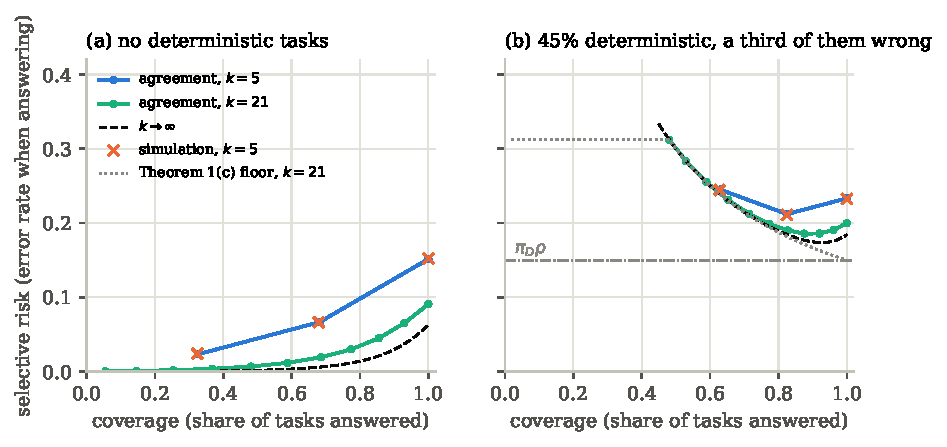
\includegraphics[width=\linewidth]{figures/risk_coverage.pdf}
\caption{Risk--coverage curves of agreement thresholding in the binary model (Proposition
\ref{prop:binary}). Noisy tasks have $A\sim\mathrm{Beta}(6,2)$. (a) Without deterministic tasks,
abstaining works: with $k=5$ runs the error rate falls from 15.2\% when answering everything to
2.3\% when answering only unanimous tasks. (b) With 30\% of tasks deterministically right and 15\%
deterministically wrong ($\pi_D=0.45$, $\rho=1/3$), the curve is inverted: with $k=21$, unanimous
answers are wrong 31.2\% of the time against 20.0\% for answering everything. Crosses: simulation
with 200{,}000 tasks. Dotted: the floor of Theorem~\ref{thm:floor}(c); dash-dotted: $\pi_D\rho$.}
\label{fig:curves}
\end{figure}

Figure~\ref{fig:curves} shows both regimes. In panel (b), more runs make the most confident
answers \emph{worse} ($24.5\%$ wrong among unanimous answers at $k=5$, $31.2\%$ at $k=21$), because
extra runs remove noisy tasks from the unanimous set and leave the systematic errors behind.
Every policy in panel (b) stays above $\pi_D\rho=0.15$, as Theorem~\ref{thm:floor}(b) requires.

\section{Breaking the floor needs label-dependent evidence}

By Lemma~\ref{lem:profile}, no amount of resampling the same agent can separate a deterministic
right answer from a deterministic wrong one. Some other observation $B$ is needed: the answer of a
second model \citep{hamidieh2026complementing}, the same agent under a perturbed prompt, or the
model's own reaction to its previous answers \citep{yadkori2024believe}.

\begin{proposition}\label{prop:second}
On deterministic tasks, let $\beta_1=\P(B=M\mid X\in D,\,C=0)$ and $\beta_0=\P(B=M\mid X\in D,\,C=1)$
be the probabilities that the second source agrees with a wrong and with a right answer. The
policy that answers a deterministic task only when $B$ agrees has risk on $D$
\[
\frac{\rho\,\beta_1}{\rho\,\beta_1+(1-\rho)\,\beta_0},
\]
which is below $\rho$ if and only if $\beta_1<\beta_0$. If $B$ is a second model, correct with
probability $b$ independently of the first in a binary task, then $\beta_0=b$, $\beta_1=1-b$.
\end{proposition}

\begin{proof}
Bayes' rule on $D$: $\P(C=0\mid B=M,X\in D)=\rho\beta_1/(\rho\beta_1+(1-\rho)\beta_0)$, and this is
below $\rho$ exactly when $\beta_1<\rho\beta_1+(1-\rho)\beta_0$, i.e.\ $\beta_1<\beta_0$.
\end{proof}

With $\rho=0.5$, an independent second model with $b=0.8$ lowers the risk on deterministic tasks to
$0.2$, and with $b=0.95$ to $0.05$. Correlated errors erode the gain: if models share the same
misconceptions, as reported across providers by \citet{ding2026agree}, then $\beta_1\approx\beta_0$
and agreement between models is as uninformative as agreement within one. Prompt perturbations
behave the same way. Removing a misleading claim from the prompt exposes errors the prompt caused
($\beta_1$ small), but not errors the agent makes for lack of knowledge, which it repeats under every
phrasing ($\beta_1\approx\beta_0$).

\section{Certification with finite samples}

Let $\lambda_1>\lambda_2>\dots>\lambda_L$ be thresholds, from most to least selective, and
$\{(S_i,C_i)\}_{i\le n}$ a labelled calibration set of i.i.d.\ tasks. For threshold $j$ let $N_j$
tasks be answered and $E_j$ of them wrong, and test $H_j:R(\lambda_j)>\alpha$ with the exact
binomial p-value $p_j=\P(\mathrm{Bin}(N_j,\alpha)\le E_j)$ \citep{clopper1934}. The
\emph{fixed-sequence} procedure \citep{angelopoulos2021ltt} rejects $H_1,H_2,\dots$ in order while
$p_j\le\delta$, returns the last rejected threshold, and abstains on everything if $p_1>\delta$.

\begin{proposition}\label{prop:ltt}
(i) $\P\big(R(\hat\lambda)>\alpha\big)\le\delta$. (ii) If every candidate policy satisfies
Theorem~\ref{thm:floor}(b) and $\pi_D\rho>\alpha$, the procedure abstains on everything with
probability at least $1-\delta$. (iii) A threshold with true risk $r<\alpha$ and coverage $c$ is
certified once about
\[
n\approx\frac{\log(1/\delta)}{c\,\mathrm{kl}(r\,\|\,\alpha)}
\]
labelled tasks are available, where $\mathrm{kl}$ is the Bernoulli Kullback--Leibler divergence.
\end{proposition}

\begin{proof}
(i) Given $N_j=n_j$, the answered tasks are i.i.d.\ and $E_j\sim\mathrm{Bin}(n_j,R(\lambda_j))$; under
$H_j$ this is stochastically larger than $\mathrm{Bin}(n_j,\alpha)$, so $\P(p_j\le\delta)\le\delta$.
A true null can be rejected only if the first true null in the sequence is rejected, which has
probability at most $\delta$. (ii) Every $H_j$ is true by Theorem~\ref{thm:floor}(b), so by (i) none is
rejected with probability at least $1-\delta$. (iii) If $E_j=rN_j$, the Chernoff bound gives
$p_j\le\exp(-N_j\,\mathrm{kl}(r\|\alpha))$, which is at most $\delta$ once
$N_j\ge\log(1/\delta)/\mathrm{kl}(r\|\alpha)$; with $N_j\approx cn$ this gives the stated $n$. It is a
heuristic because $E_j$ fluctuates around $rN_j$.
\end{proof}

For $r=5\%$, $\alpha=10\%$, $c=0.5$ and $\delta=0.1$ the rule gives about 276 labelled tasks; for
$r=2\%$ and $\alpha=5\%$, about 379. Figure~\ref{fig:cert} runs the procedure on two populations
with $k=5$. When $\pi_D\rho=0.02<\alpha$, the certified coverage grows with $n$ and reaches the best
feasible coverage, 0.80, by $n\approx 800$; the empirical violation rate never exceeds 2.8\%,
below $\delta=10\%$. When $\pi_D\rho=0.15>\alpha$, the procedure certifies nothing at any $n$, as
Proposition~\ref{prop:ltt}(ii) predicts. The guarantee holds in both cases; in the second it is
honest and useless.

\begin{figure}[t]
\centering
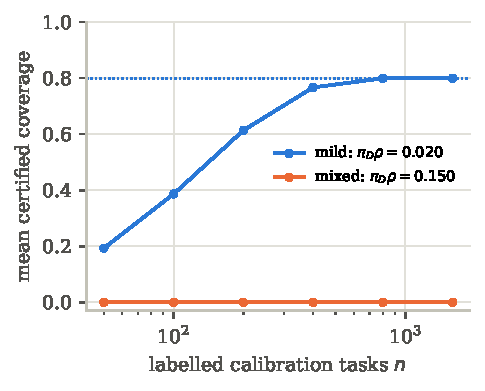
\includegraphics[width=0.52\linewidth]{figures/certification.pdf}
\caption{Fixed-sequence certification at $\alpha=\delta=0.1$ with $k=5$, 1{,}000 calibration sets
per point. ``mild'': 35\% of tasks deterministically right, 2\% deterministically wrong. ``mixed'':
the population of Figure~\ref{fig:curves}(b). Dotted: the largest coverage whose true risk is at
most $\alpha$.}
\label{fig:cert}
\end{figure}

\section{How many runs, how many tasks}

Evaluating an agent raises the same structure from the other side. Let $e(x)=\P(\text{run
wrong}\mid X=x)$ and $\theta=\E\,e(X)$, and estimate $\theta$ by the mean error over $I$ tasks with $k$
runs each.

\begin{proposition}\label{prop:eval}
With $\mathrm{ICC}=\operatorname{Var}e(X)/(\theta(1-\theta))$, the intra-task correlation of
run errors,
\[
\operatorname{Var}\hat\theta=\frac{\theta(1-\theta)}{Ik}\,\big(1+(k-1)\,\mathrm{ICC}\big).
\]
The binomial interval that treats all $Ik$ runs as independent has asymptotic coverage
\[
2\Phi\Big(z\big/\sqrt{1+(k-1)\,\mathrm{ICC}}\Big)-1\quad\text{instead of}\quad 2\Phi(z)-1.
\]
If a new task costs $\kappa$ times a run, the variance for a fixed budget is minimised by
\[
k^\star=\sqrt{\kappa\,(1-\mathrm{ICC})/\mathrm{ICC}}
\]
runs per task. $\mathrm{ICC}=1$ if and only if $e(X)\in\{0,1\}$ almost surely, that is, if every
task is deterministic.
\end{proposition}

\begin{proof}
By the law of total variance, $\operatorname{Var}\hat\theta=\frac1I\big(\operatorname{Var}e(X)+
\E[e(X)(1-e(X))]/k\big)$, and $\theta(1-\theta)=\operatorname{Var}e(X)+\E[e(X)(1-e(X))]$; rearranging
gives the design effect \citep{kish1965survey}. The coverage follows from the ratio of the true and
assumed standard errors. For the allocation, minimise
$(\operatorname{Var}e+\E[e(1-e)]/k)/I$ subject to $I(\kappa+k)=B$. Finally $\E[e(1-e)]=0$ if and only
if $e\in\{0,1\}$ almost surely.
\end{proof}

\begin{table}[t]
\centering
\small
\begin{tabular}{lccc}
\toprule
& $k=3$ & $k=5$ & $k=10$\\
\midrule
$\mathrm{ICC}=0.2$ & 90.2\% & 85.6\% & 75.9\%\\
$\mathrm{ICC}=0.5$ & 83.4\% & 74.2\% & 59.7\%\\
$\mathrm{ICC}=0.8$ & 77.6\% & 66.1\% & 50.6\%\\
$\mathrm{ICC}=1.0$ & 74.2\% & 61.9\% & 46.5\%\\
\bottomrule
\end{tabular}
\caption{Actual coverage of a nominal 95\% binomial interval that counts runs as independent.}
\label{tab:naive}
\end{table}

Table~\ref{tab:naive} shows how quickly the naive interval fails; the ``mixed'' population of
Figure~\ref{fig:curves} has $\mathrm{ICC}=0.55$. Resampling the tasks, not the runs, restores
coverage \citep{miller2024errorbars}. The ICC is estimable from any evaluation with two or more runs
per task, using $\E[Z_tZ_s]=\E[e(X)^2]$ for two runs $t\neq s$ of the same task.

The ICC links the two halves of this note. It is the share of error variance that lies
\emph{between} tasks. A high ICC makes extra runs nearly worthless for evaluation ($k^\star\to 0$),
and it is also the regime in which runs agree with each other whether or not they are right. At
the extreme, $\mathrm{ICC}=1$ means $\pi_D=1$ and $\rho=\mu$, and Theorem~\ref{thm:floor}(a) gives
$R(\varphi)\ge\mu$ for every label-invariant policy: no abstention rule built on resampling can do
better than answering everything.

\section{Related work}

Empirical studies document low-entropy errors and their cost for selective prediction
\citep{phillips2026entropy,kossen2024probes}, and propose cross-model disagreement
\citep{hamidieh2026complementing} or iterative prompting \citep{yadkori2024believe} as epistemic
signals. \citet{ding2026agree} audits self-consistency and finds confident errors shared across
providers. \citet{mouzouni2026blackbox} combines self-consistency with conformal prediction sets
and notes that the majority answer is biased when the per-run accuracy is at most one half.
On the certification side, \citet{kotte2026crc} gives a score-agnostic feasibility bound for
conformal risk control, which is the upper end of our certifiable window, and
\citet{akter2025lift} bounds the abstention needed when the evidence carries little mutual
information about correctness. Our results are specific to the label-invariant class but use no
assumption on the score's quality: they hold for the best possible label-invariant score and an
infinite calibration set. Selective classification with guaranteed risk goes back to
\citet{geifman2017selective}; risk-controlling calibration to \citet{angelopoulos2021ltt} and
\citet{angelopoulos2024crc}, with abstention for LLMs in \citet{yadkori2024conformal}.

\section{Limitations and open questions}

\begin{itemize}[leftmargin=*,itemsep=2pt]
\item \textbf{Independent runs.} Runs are assumed i.i.d.\ given the task. Caching, fixed seeds or
temperature zero make runs identical, which only enlarges $D$.
\item \textbf{Exact determinism.} The theorem uses tasks with a point-mass output; the remark on
$D_\epsilon$ quantifies near-determinism, but how much of a real agent's error mass sits near
$a_1=1$ is an empirical question.
\item \textbf{Label-invariant scores only.} Token probabilities, verbalised confidence, verifiers
and probes are outside the class and can, in principle, beat the floor; whether they do on
systematic errors needs measurement.
\item \textbf{No experiments on real agents.} All numbers here come from synthetic populations.
The natural next step is to estimate $\pi_D$, $\rho$ and the ICC on agent benchmarks with several
runs per task, where they would predict, before any calibration, which risk levels can be
certified.
\end{itemize}

\paragraph{Reproducibility.} Code for every closed form, the simulations and the figures is in
the repository accompanying this note; \texttt{tests/test\_theory.py} checks
Theorem~\ref{thm:floor} on 300 random populations and policies and each proposition against Monte
Carlo.

\renewcommand{\bibfont}{\small}
\setlength{\bibsep}{3pt}
\bibliographystyle{plainnat}
\bibliography{refs}

\end{document}
